\section{Enablers}
\label{sec:enablers}

This section describes the enablers, which are the prerequisites that the innovating company, i.e., LinkedIn, brings
to the table and that must match with the customer perspective that we introduced in the previous section. Enablers
can be based on the uniqueness of the company (i.e., its offering can not easily be copied by competitors) or on
operational excellence (i.e., the company is able to provide its offering at a significantly lower cost than its
competitors). The enablers are added to the company-side of the \emph{Value Proposition Canvas}
\citep{osterwalderValuePropositionDesign2014}.

\subsection{Uniqueness}
\label{subsec:uniqueness}

LinkedIn can provide a new service, i.e., \textit{Career Counseling as a Service} (CCaaS), based on its
unique position in the market, its broad access to career and job data, and access to state-of-the-art 
AI technology and machine learning algorithms.

\subsubsection{Market Position}

LinkedIn is the world's largest professional network with more than 900 million members in over 200 countries
worldwide \citep{linkedinLinkedInPressromUs2023}. LinkedIn has a unique position in the market, see e.g.,
\cite{kaserAIpoweredCareerCounseling2023,99firmsLinkedInStatistics20232023}: 

\begin{itemize}
    \item LinkedIn's user base encompasses 900 million users (January 2023)
    \item LinkedIn is used by 49 million users weekly
    \item 365 million users have skills data on their profile (44\% of jobs filled with
        LinkedIn already use skills data as part of the recruiting)
    \item 50 million job searches per week (the widest reach in many Western countries)
\end{itemize}

\subsubsection{Access to Data}

LinkedIn is one of very few companies that has access to the data of such a massive user base, including
very granular data on users' education, work experience, skills, and interests. LinkedIn also has access
to data on companies and their organizational structures, job advertisements, and hiring practices. This
data is a valuable resource for LinkedIn and can be used to train AI-based tools, e.g., job recommendation
systems, career path recommendation systems, and career counseling systems. Due to the combination of the
larger amount of data and more granular data, LinkedIn is in a unique position to train better AI algorithms
than its competitors. Another less obvious data advantage is the graph structure of the data in LinkedIn,
where users are connected to other users, to companies via work experiences, and to schools via education.
This graph structure can be used to train graph-based machine learning algorithms that can provide better
recommendations than traditional machine learning algorithms due to overcoming data sparsity and cold start
problems \citep{zhangRecommendingGraphsComprehensive2023}.

\subsubsection{Access to Technology and AI}

LinkedIn is part of Microsoft, one of the world's largest technology companies. Microsoft has invested heavily
in artificial intelligence (AI) and machine learning (ML) in recent years, including owning a stake in the hottest
of the AI companies, i.e., OpenAI \citep{openaiAnnouncementOpenAIMicrosoft2023}. Microsoft also owns GitHub and has
already proved that it can successfully integrate one of its companies with the offerings from OpenAI. In particular,
Microsoft and OpenAI have jointly developed GitHub Copilot, an AI-based code assistant that helps developers to write
better code, leveraging the huge database of GitHub and the AI know-how from OpenAI \citep{novetMicrosoftOpenAIHave2021}.
LinkedIn has similarly access to Microsoft's and OpenAI's AI and ML technologies. 

\subsection{Operational Excellence}

\subsubsection{Master of Scale}

LinkedIn has successfully mastered scaling challenges in the past, including a phase of hypergrowth. As a result
LinkedIn has a proven track record in architecting scalable software systems based on a microservices approach
\citep{linkedinBriefHistoryScaling2015}. 

\subsubsection{Master of Speed}

LinkedIn suffered major architectural challenges after its IPO. Subsequently, LinkedIn engineering teams mastered a
revamp of its systems architecture and developer tooling, putting them ahead of competitors in terms of speed of
experimenting, iterating and new feature delivery \citep{vanceOperationInVersionCode2013}.

\subsubsection{Master of Cost}

\cite{floereckeSuccessFactorsSaaS2018} researched success factors for software-as-a-service (SaaS) business models and
found the main one to be that \textit{``SaaS service[s] should be developed as a system comprising modular microservices
in order to meet the desired requirements in terms of cost advantages, performance and scalability''}. Accordingly, CCaaS
should be designed as a system of modular microservices that are offered via an API layer. Further, adoption by career
counselors can be facilitated via a marketplace for career counselors and low/no-code solutions. This allows for leveraging
CCaaS services without fully, costly technical integration of the API.

\subsection{Products \& Services}

The services provided as part of CCaaS can be offered as a bundle or individually. Based on the microservices
approach, the counseling service providers can choose which API endpoints they want to use and integrate into 
their offerings. LinkedIn's CCaaS offering should encompass the following services:

\begin{itemize}
    \item\textbf{AI Models:}
        Build and offer the AI models for career counseling based on the data that LinkedIn has access to, including
        user profiles, skills, educations, job postings, and feedback data from career counselors participating in CCaaS.
    \item\textbf{API Layer:}
        Provide all CCaaS services as reliable, highly available, and scalable API endpoints.
    \item\textbf{Career Counselor Matchmaking:}
        Matchmaking between career counselors band the clients based on their user profile data, the counselors' past
        customers, geographic proximity, and other factors.
    \item\textbf{Skills Assessment:} 
        Skills assessment based on user profile data from LinkedIn, including gap analysis.
    \item\textbf{Job Search \& Recommender:}
        Search and recommend jobs based on similarity with the user's profile leveraging word embeddings and graph embeddings.
    \item\textbf{Writing Assistant:}
        Provide a writing assistant for preparing CVs and cover letters for job applications using generative AI
        tools.
    \item\textbf{Career Path Recommender:}
        Recommend career paths based on the similarity of the user's profile and  similar users' career paths
        leveraging graph embeddings.
    \item\textbf{Training Recommender:}
        Recommend trainings to a user based on profile and chosen career path (help user fill skill gaps
        required for career path).
\end{itemize}

\subsection{Gain Creators}

Gain creators describe how the products and services of a company create gains for the customer. In the
case of CCaaS, the gain creators are the services that are provided (via the career counselors) to the end
customers like Sarah. Gain creator should match the gains introduced in the customer perspective.

\begin{itemize}
    \item Enable career counselors to provide semi-automated but highly personalized career counseling
    \item Provide insights and better recommendations for career paths, jobs, and trainings through superior AI models
    \item Enable self-service career counseling platforms
\end{itemize}

\subsection{Pain Relievers}

Similarly to gain creators, pain relievers describe how the products and services of a company relieve
the pains that are experienced by the customers.

\begin{itemize}
    \item Reduce costs by shared AI models and shared infrastructure
    \item Increase efficiency in career counseling 
    \item Provider better insights and recommendations through broader and more granular data
\end{itemize}

\begin{figure}[h!]
    \centering
    \caption{The full Value Proposition Canvas with customer- and company side (background illustration adapted from Strategyzer.com).}
    \label{fig:vpc_full}
    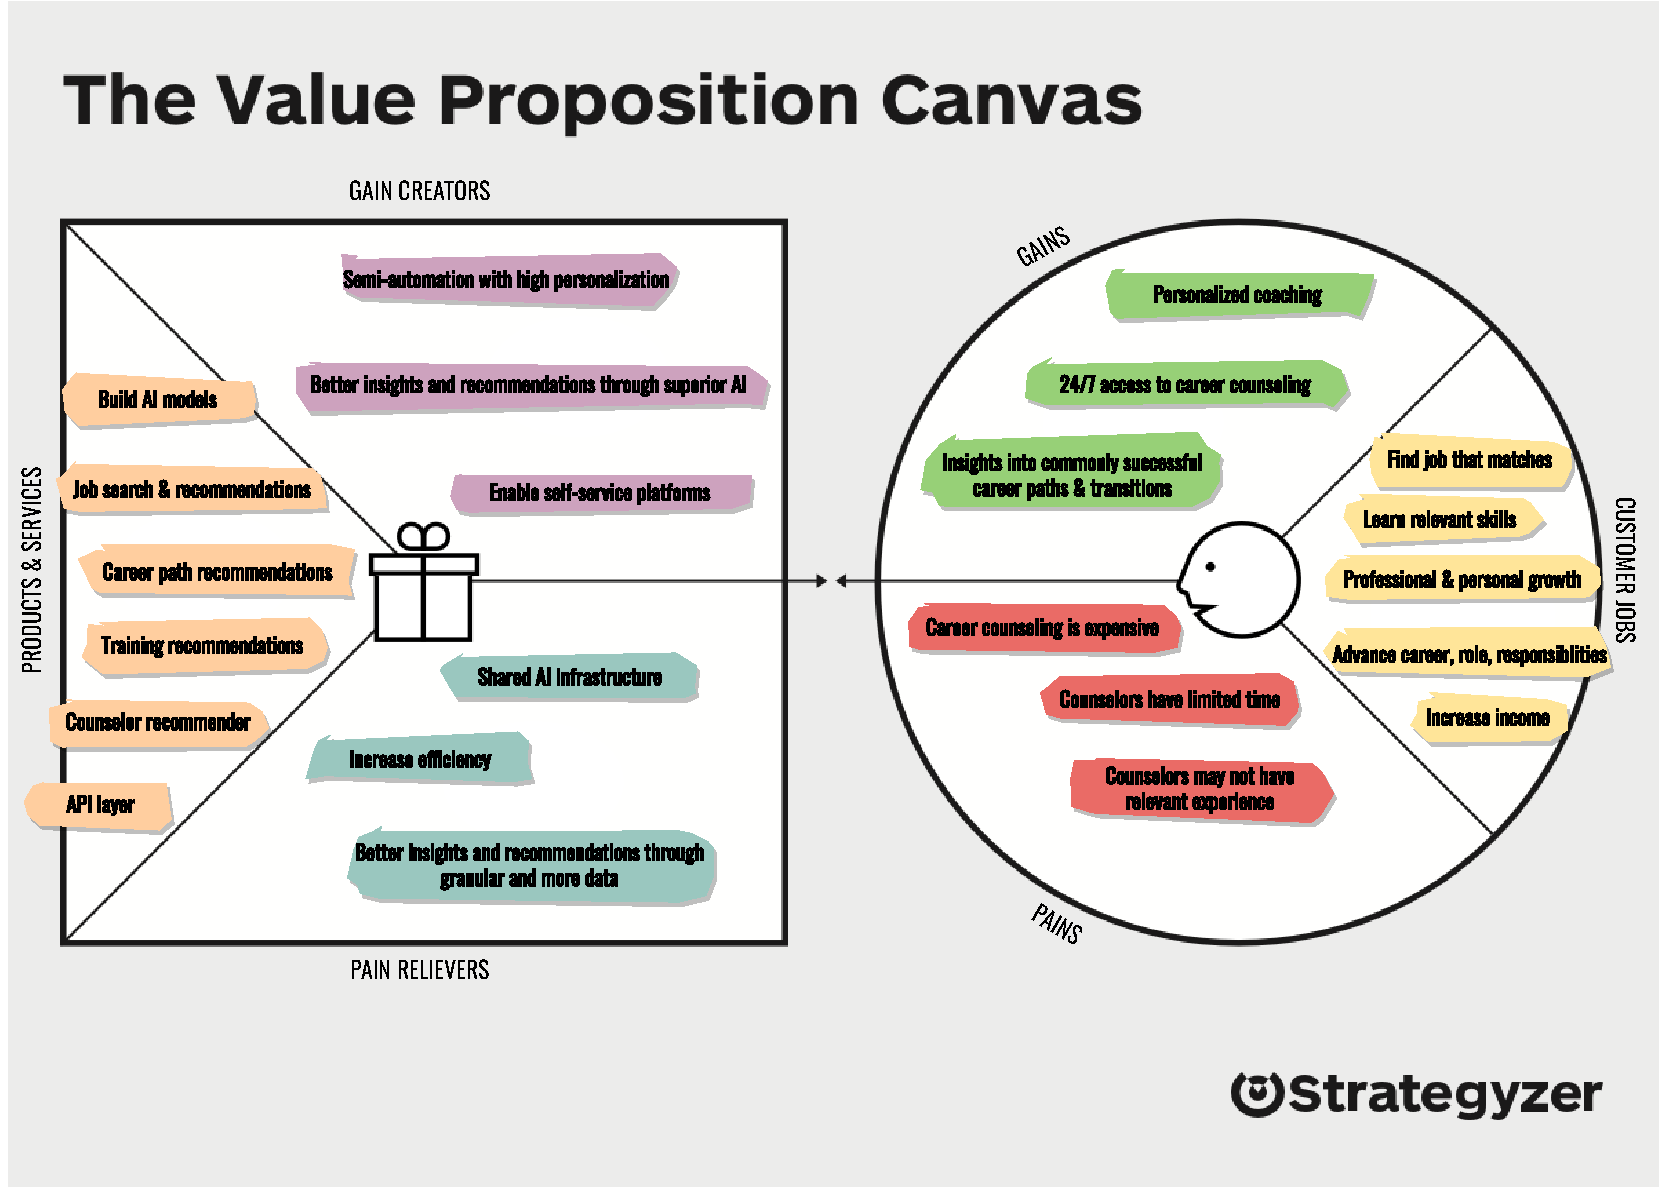
\includegraphics[width=\linewidth]{vpc_full.pdf}
\end{figure}

\subsection{Customer Centricity: Addressing Customer Needs}

By combining the customer-side and the company-side of the value proposition canvas, we can identify
the services that relate to customer jobs via either gains and gain creators or pains and pain relievers.
This is illustrated in Figure \ref{fig:vpc_full}. Table \ref{tab:vpc} summarizes how the services connect
with the customer jobs and thus ensure a high customer-centricity of the business model that we will develop
in the next section. Some common gains and pains and matching gain creators and pain relievers are listed as 
part of the jobs to be done.

\begin{table}[htb]
    \caption{
        Connecting customer jobs with services via gains / gain creators and pain / pain relievers.
    }
    \label{tab:vpc}

    \tiny
    \renewcommand{\arraystretch}{1.1}
    \small\centering
    \setlength\tabcolsep{8pt}
    \begin{tabularx}{\linewidth}{m m m m}
        \toprule
        \textbf{Customer Job} & \textbf{Gains / Pains} & \textbf{Creators / Relievers} & \textbf{Services} \\
        \toprule

        Find job that matches &
            Counselor may not have relevant experience &
            Better insights through more \& granular data &
            Job search \& recommendations; writing assistant for CV and cover letter\\ 
        \midrule
        
        Learn relevant skills &
            Insights into commonly successful career paths &
            Better insights through superior AI &
            Skills assessment; training recommendations; career path recommendations\\ 
        \midrule

        Professional \& personal growth &
            Personalized coaching &
            Semi-automation with high personalization &
            Job recommendations; training recommendations; career path recommendations\\ 
        \midrule

        Advance career, responsibility, role &
            Personalized coaching &
            Better insights through superior AI; better insights through more \& granular data&
            Counselor recommendations; career path recommendations; training recommendations \\ 
        \midrule

        Increase income &
            Career counseling is expensive; counselors have limited time; 24/7 access to counseling &
            Self-service platform; increase efficiency; shared AI infrastructure &
            Counselor recommendations; career path recommendations \\ 
        \bottomrule
    \end{tabularx}
\end{table}

\subsection{Value Co-Creation Through Collaboration}

According to \citet{griederDigitalEcosystemHow2019}, most companies are still working on management theories 
and principles that were developed in the industrial age. They continue to argue that in the digital age,  
companies should join a digital ecosystem where value is co-created through collaboration of different 
participants. In the following we develop how value is co-created in the AI-based career counseling ecosystem
with LinkedIn's CCaaS as an important component.

The direct customers of LinkedIn's new CCaaS service will be independent career counselors, counseling companies, 
counselors at educational institutions and job centers. Further, new start-up companies may emerge taking advantage
of the CCaaS API and potentially combining it with other offerings, such as integrating with assessment platforms 
or learning platforms (Coursera, Udemy, etc.). However, the end customers of the CCaaS service are the clients of
the counselors that we introduced in the customer perspective. As LinkedIn is not specialized in career counseling
but is a social network that connects professionals, it is not its core business to provide career counseling.
Therefore, LinkedIn needs to collaborate with these specialized counselors that can provide specialized career
counseling services. Also, career counselors may work at different locations around the world. For instance, our
persona Sarah may wish to receive personal career coaching on-site at her university in Zurich. The combination of
the CCaaS offering and counselors specialized knowledge, experience and geographical distribution will provide
the end customers with a unique value proposition that is not available today, with LinkedIn and its CCaaS offering
at the center of the value co-creation network.

LinkedIn sits atop a mountain of valuable career data from its 900+ million members. Its contribution to the value 
creation is to provide highly specialized, machine learning based services. For instance, LinkedIn can provide a
service that recommends career counselors to its members based on their profile data. Career counselors can access
machine learning based recommendations of career paths for their clients using the CCaaS API layer. LinkedIn could
design the CCaaS API layer in a way that career counselors could actively or passively leave feedback on the job
recommendations and career path recommendations provided by LinkedIn, thereby helping LinkedIn to collect additional,
refined data which are useful to further improve its machine learning models. Both, LinkedIn and career counselors,
thereby actively contribute to a higher value creation for the clients that was not possible before. The CCaaS API
layer presents a \textit{win-win-win} situation for all three engaged parties: LinkedIn, the counselors and the
counseling clients.
\newline

\noindent In Section \ref{sec:business_model}, we will develop a business model for LinkedIn's CCaaS offering.